\documentclass{dsfe}

%%%%%%%%%%%%%%%%%%%%%%%%%%%%%%%%%%%%%%%%%%
\usepackage{txfonts}
\def\typeofarticle{Research article}
\def\currentvolume{xx}
\def\currentissue{x}
\def\currentyear{2025}
\def\currentmonth{Received date xx-xx, Accepted date xx-xx}
\def\ppages{xxx--xxx}
\def\DOI{10.3934/DSFE.2025xxx}
\def\Received{}
\def\Revised{}
\def\Accepted{}
\def\Published{}
\usepackage{lineno}

\newcommand{\ep}{\varepsilon}
\newcommand{\eps}[1]{{#1}_{\varepsilon}}


%\numberwithin{equation}{section}
%\DeclareMathOperator*{\essinf}{ess\,inf}


\begin{document}
%\linenumbers

\title{Enhancing Cryptocurrency Price Prediction Using Hybrid Regression and RNN Models}

\author{%
  Wiem Ben Romdhane\affil{1}\corrauth,
  and  Heni Boubaker\affil{1,2}
}

% \shortauthors is used in copyright information in the end of the paper
\shortauthors{the Author(s)}

\address{%
  \addr{\affilnum{1}}{LaREMFiQ, IHEC , University of Sousse - Tunisia}
  \addr{\affilnum{2}}{Departement of Quantitative Methods and Economics, IHEC, University of Sousse - Tunisia}}

% corresponding author
\corraddr{Email wiembr@gmail.com}

\begin{abstract}
The volatile and complex nature of cryptocurrency markets demands advanced forecasting techniques to enhance predictive accuracy. This study explores the efficacy of hybrid models combining Recurrent Neural Networks (RNNs)—specifically Long Short-Term Memory (LSTM) and Gated Recurrent Unit (GRU)—with statistical methods like Ordinary Least Squares (OLS) and simple averaging for forecasting Bitcoin (BTC), Ethereum (ETH), and Litecoin (LTC) prices. Using daily closing price data from 2018 to 2025, we evaluate model performance via Root Mean Squared Error (RMSE), Root Mean Absolute Error (RMAE), and Mean Absolute Percentage Error (MAPE). Empirical results reveal that the combined OLS model excels for BTC and LTC, achieving the lowest error metrics (e.g., MAPE of 2.693\% for BTC), while LSTM outperforms for ETH (RMSE: 114.52). Hybrid approaches demonstrate robustness, balancing the temporal learning strengths of RNNs with the stability of statistical methods. Visual comparisons further validate the models’ alignment with actual price trends. This research underscores the potential of hybrid models to mitigate volatility challenges, offering actionable insights for investors and advancing methodological innovation in cryptocurrency forecasting.
%\textbf{}
\end{abstract}

\keywords{ Cryptocurrency Forecasting; OLS; LSTM; GRU; Combined models; Time series analysis
%\textbf{(5 to 10 keywords)}
}

\maketitle

\section{Introduction}

The rapid rise of cryptocurrencies, such as Bitcoin, Ethereum, and Litecoin, has revolutionized the financial landscape, offering decentralized and secure alternatives to traditional currencies. However, the highly volatile and unpredictable nature of cryptocurrency markets poses significant challenges for investors, policymakers, and researchers. Accurate forecasting of cryptocurrency prices is crucial for making informed decisions, yet the complexity of these markets, driven by factors such as market sentiment, global economic trends, and technological advancements, makes this task particularly challenging.

In recent years, machine learning and deep learning techniques have emerged as powerful tools for financial time series forecasting. Among these, Recurrent Neural Networks (RNNs), particularly Long Short-Term Memory (LSTM) networks and Gated Gated Recurrent Unit (GRU), have shown remarkable success in capturing temporal dependencies and patterns in sequential data. LSTMs networks are a specialized form of Recurrent Neural Networks tailored for handling time-dependent data, making them particularly effective for tasks like time series forecasting. GRUs is an advanced variant of Recurrent Neural Networks specifically engineered to overcome certain shortcomings of traditional RNNs. A key issue with standard RNNs is the "vanishing gradient problem," where the gradients responsible for updating the network's weights during training diminish to such an extent that the model struggles to learn long-term patterns in the data. GRUs mitigate this problem by incorporating gating mechanisms that allow for more efficient information flow over time.

However, the inherent noise and non-linearity of cryptocurrency data often limit the performance of standalone models. To address this, researchers have increasingly turned to combined or hybrid models that integrate the strengths of multiple approaches, such as combining RNNs with statistical methods, optimization algorithms, or other machine learning techniques.

This research paper explores the potential of combined models that leverage RNNs for forecasting cryptocurrency prices. By combining RNNs with complementary methodologies, such as ordinary least square (OLS) and simple average techniques, the study aims to enhance prediction accuracy and robustness. Through empirical analysis and comparative evaluation, this research seeks to contribute to the growing body of knowledge on cryptocurrency forecasting, offering insights into the development of more reliable and adaptive predictive models.

\section{Related works}
Predicting cryptocurrency prices has become a topic of great interest in recent years, driven by the increasing significance of digital assets in global financial markets. Due to the highly volatile and non-linear nature of cryptocurrency markets, conventional statistical models often struggle to effectively capture the intricate patterns and dependencies within the data. Consequently, researchers have increasingly adopted machine learning and deep learning approaches, particularly Recurrent Neural Networks (RNNs), to enhance forecasting accuracy. In this context, hybrid models that combine RNNs with other techniques have demonstrated significant potential in overcoming the limitations of standalone models \citep{oyewola2022, ferdiansyah2023, garcia2024}.

In their paper, \citep{zhang2021} proposed the weighted and attentive memory convolutional neural network (WAMC) to enhance cryptocurrency price prediction accuracy. The model integrates a GRU for attentive memory, a channel-wise weighting module to capture interdependencies among cryptocurrencies, and a CNN to extract local temporal features. Tested on ETH and BTC, the WAMC model achieved RMSE scores of 9.70 and 1.37, respectively, demonstrating its potential for accurate price forecasting. \citep{aghashahi2023} explore how integrating technical attributes, such as price-related and lagged features, into neural networks enhances prediction accuracy, ultimately influencing profitability. They evaluate model performance and examine how specific configurations contribute to reliable and effective predictions for profitable trading. \citep{garcia2024} predict the volatility of major cryptocurrencies using Generalized Autoregressive Conditional Heteroskedasticity (GARCH) models, Multilayer Perceptron (MLP), Long Short-Term Memory (LSTM), and hybrid LSTM-GARCH models. They conclude that MLP models yield the best predictive performance while their accuracy is not statistically distinct from LSTM and LSTM-GARCH models based on the Diebold–Mariano test. \citep{seabe2023} employ three deep learning techniques -LSTM, GRU and Bi-LSTM to predict the price of the top three cryptocurrencies BTC, ETH and LTC and they find that the Bi-LSTM model delivered the most accurate predictions across all three currencies.  The study of \citep{xiang2024} explores LSTM, Neural Networks, and Deep Learning (CNN) for predicting cryptocurrency prices, utilizing technical indicators and sentiment analysis. The hybrid model combining these techniques achieves the highest predictive accuracy for cryptocurrencies like Bitcoin, Ethereum, and Binance Coin, as measured by RMSE. Challenges include adaptability to market volatility and data noise, with future improvements potentially incorporating external factors and interdisciplinary approaches. The research highlights the potential of hybrid deep learning models in improving cryptocurrency valuation and risk management strategies.
The study of \citep{amberkhani2025} explores multiple machine learning and deep learning models and fbProphet, to improve cryptocurrency price forecasting. XGBoost and the LSTM-GRU hybrid demonstrated strong performance, though challenges like overfitting remain.  The research of \citep{hoa2025} proposes a novel hybrid model that integrates one-dimensional convolutional neural networks (1D-CNN) with long short-term memory (LSTM) networks to predict Ethereum's closing prices. The experimental findings reveal that the hybrid model achieves superior performance compared to baseline models, highlighting its potential to enhance forecasting accuracy in the highly volatile cryptocurrency markets. \citep{hadfi2025}  introduce a novel methodology for cryptocurrency price prediction by automating hyperparameter selection and analyzing interconnections among cryptocurrencies. The approach integrates deep learning techniques, including RNNs and LSTMs, with the Genetic Algorithm (GA) to optimize model parameters. By automating the hyperparameter tuning process and accounting for the relationships between different cryptocurrencies, the method significantly improves forecasting accuracy. This innovative solution is designed to address the challenges of dynamic and interconnected cryptocurrency markets, providing practical benefits for investors and contributing to academic advancements in the field. \citep{kiranmai2025} develop a dynamic forecasting model using ensemble methods (GBR, RFR, SVR, MLP) to predict top 15 cryptocurrencies' prices, optimizing parameters for accuracy. Statistical and econometric models are evaluated, with validation curves enhancing prediction precision. The ensemble model leverages machine learning to improve forecasting performance.  The study of \citep{amirshahi2025}  extracts sentiment from cryptocurrency-related tweets using an ensemble of three pre-trained language models. Twenty model versions were evaluated on 27 top cryptocurrencies, incorporating historical sentiment and price data for predictions. The model's flexible input layer adapts to different cryptocurrencies, optimizing accuracy. Findings indicate longer input sequences yield the most accurate predictions on average.
\section{Materials and method}
\subsection{Overview of LSTM and GRU Models}
\subsubsection{LSTM Model}
Long Short-Term Memory (LSTM) is an advanced recurrent neural network (RNN) architecture that integrates gating mechanisms to address the limitations of traditional RNNs, such as vanishing gradient problems \citep{hochreiter97}. Specifically designed for sequential data, LSTM excels at capturing both short-term and long-term dependencies within time series, making it highly effective for tasks requiring temporal modeling [14]. Each LSTM unit consists of recurrent cells that maintain two key internal states over time: the cell state $c_t$, which stores long-term information, and the hidden state $h_t$, which captures short-term context. These cells are governed by nonlinear gating mechanisms—input, forget, and output gates—that regulate the flow of information. The input gate determines which new information to store, the forget gate decides what to discard from the cell state, and the output gate controls the information passed to the next time step. This dynamic gating structure enables LSTMs to adaptively learn and model complex temporal patterns, making them particularly suited for applications involving time series forecasting, natural language processing, and other sequential data tasks.
\begin{figure}[H]
\begin{center}
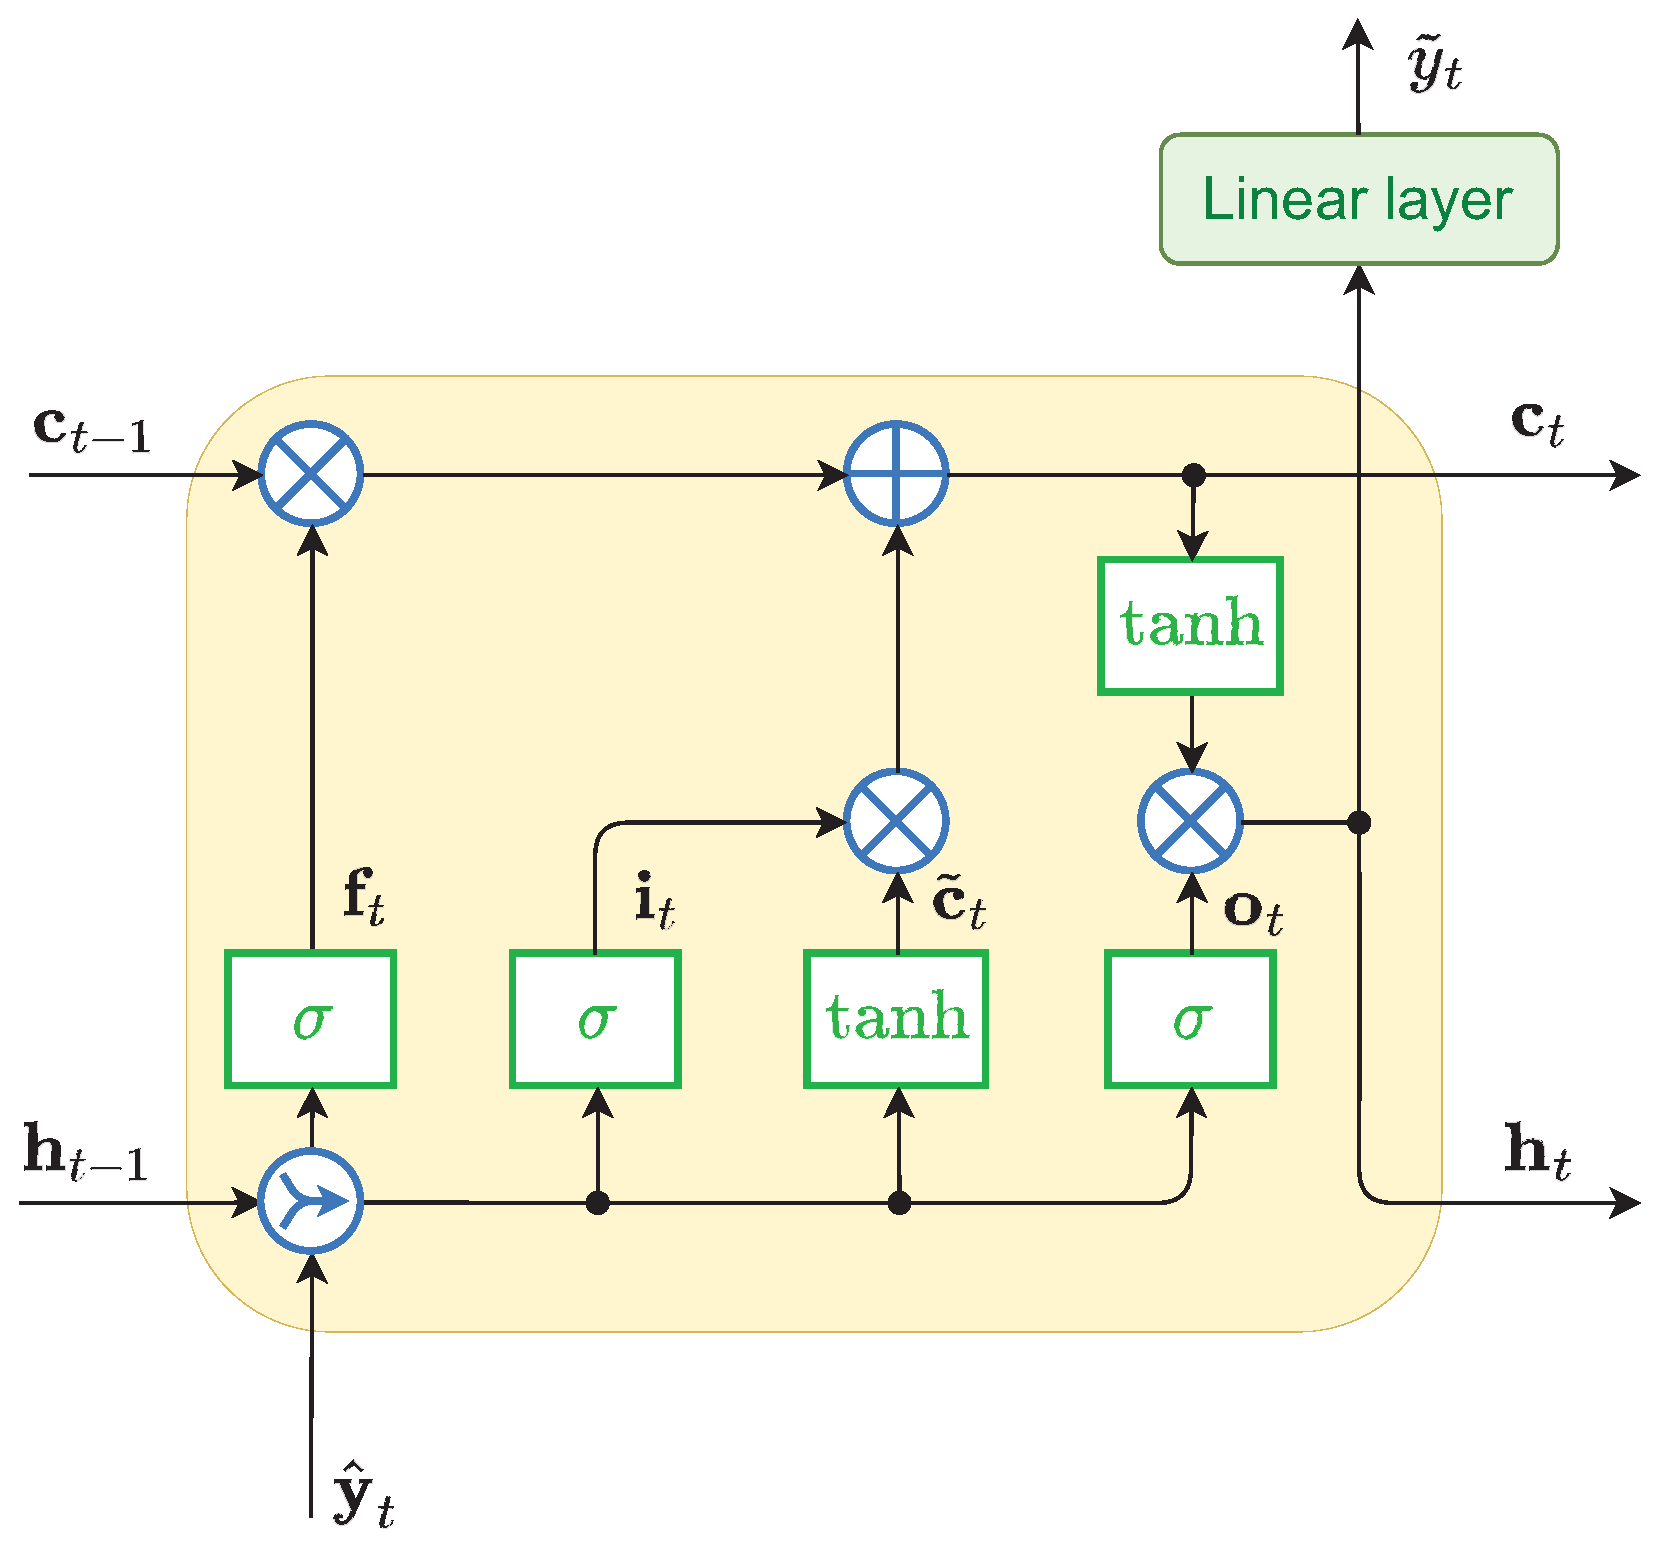
\includegraphics[scale=0.2]{lstmCell.png}
\caption{LSTM model - Source: \citep{dudek2023}.}\label{lstm_cell}
\end{center}
\end{figure}
In \autoref{lstm_cell}, the architecture of an LSTM block is illustrated, showcasing its key components: the input signal $x_t$, the output $h_t$, and the activation functions that govern its operations. The LSTM block is designed to manage information flow through a series of gating mechanisms, which are critical for its ability to learn and retain long-term dependencies. The input gate plays a pivotal role in determining which elements of the incoming data $x_t$ should be stored in the cell state $c_t$, ensuring that only relevant information is preserved. Conversely, the output gate regulates the release of information from the cell state to the hidden state $ht$, controlling what is passed on to subsequent time steps. These gates, along with the forget gate (which decides what information to discard from the cell state), enable the LSTM to dynamically adapt to the temporal structure of the data.

The forward training process of an LSTM network can be mathematically described by the following set of equations, which define the operations within a single LSTM unit at time step $t$:
\begin{enumerate}
\item \textbf{Forget Gate:}
\begin{equation}
f_t  =  \sigma\left(W_f [h_{t-1}, x_t]+b_t \right)
\end{equation}
\item \textbf{Input Gate:}
\begin{align}
i_t  =  & \sigma\left(W_i \dot [h_{t-1}, x_t]+b_i \right)\\
\tilde{c}_t = & \tanh\left(W_c \dot [h_{t-1}, x_t]+b_c\right)
\end{align}
Here, $i_t$ controls the update of the cell state, and $\tilde{c}_t$ represents the candidate values for the new cell state.
\item \textbf{Cell State Update:}
\begin{equation}
c_t  =  f_t \odot c_{t-1}+i_t \odot \tilde{c}_t
\end{equation}
The cell state $c_t$ is updated by combining the information retained from the previous state and the new candidate values.
\item \textbf{Output Gate:}
\begin{align}
o_t  = &  \sigma\left(W_o \dot [h_{t-1}, x_t]+b_o \right)\\
h_t  = &  o_t\odot \tanh(c_t)
\end{align}
The output gate $o_t$ determines the portion of the cell state $c_t$ that will be output as the hidden state $h_t$.
\end{enumerate}
These equations collectively enable the LSTM to process sequential data effectively, balancing the retention of long-term information with the incorporation of new inputs. The gating mechanisms ensure that the network can adaptively learn and model complex temporal patterns, making LSTMs a powerful tool for tasks such as time series forecasting, natural language processing, and more.

\subsubsection{GRU Model}
Gated Recurrent Units (GRUs) are a specialized variant of Recurrent Neural Networks (RNNs) introduced by \citep{chao2014} as a streamlined and computationally efficient alternative to Long Short-Term Memory (LSTM) networks. Like LSTMs, GRUs are designed to process input sequences of variable lengths and maintain a hidden state that encapsulates historical information, enabling them to model temporal dependencies effectively. However, GRUs achieve this with a more simplified architecture, utilizing only two gating mechanisms: an update gate and a reset gate. The update gate controls how much of the previous hidden state should be retained and how much new information should be incorporated, while the reset gate determines which portions of the past information should be discarded. This reduction in gating mechanisms eliminates the need for a separate cell state, as used in LSTMs, resulting in a more compact and computationally efficient model.

The simplified design of GRUs offers several advantages, including faster training times and reduced complexity, making them particularly suitable for scenarios where computational resources are limited or real-time processing is required. Despite their architectural simplicity, GRUs have demonstrated performance comparable to LSTMs across a wide range of sequence modeling tasks, such as natural language processing, speech recognition, and time series forecasting \citep{yang2020}. This balance of efficiency and effectiveness has solidified GRUs as a popular choice for researchers and practitioners seeking robust yet lightweight solutions for sequential data analysis. The architecure of a GRU block is illustred in \autoref{gru_cell}.
\begin{figure}[H]
\begin{center}
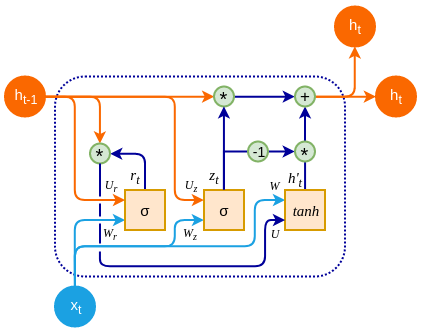
\includegraphics[scale=0.8]{GRU.png}
\caption{GRU model - Source: \citep{vasilev2019}.}\label{gru_cell}
\end{center}
\end{figure}
Below are the key equations that define the operations within a GRU unit at time step $t$:
\begin{enumerate}
\item \textbf{Reset Gate:}
\begin{equation}
r_t=\sigma\left(W_r \dot [h_{t-1}, x_t]+b_r \right)
\end{equation}
The reset gate $r_t$ determines how much of the previous hidden state $h_{t-1}$ should be ignored when computing the candidate activation.
\item \textbf{Update Gate:} 
\begin{equation}
z_t=\sigma\left(W_z \dot [h_{t-1}, x_t]+b_z \right)
\end{equation}
The update gate $z_t$ balances the influence of the previous hidden state $h_{t-1}$ and the candidate hidden state $\tilde{h}_t$.
\item \textbf{Candidate Hidden State:}
\begin{equation}
\tilde{h}_t=\tanh\left(W_h \dot [r_{t}\odot h_{t-1} , x_t]+b_h \right)
\end{equation}
The candidate hidden state $\tilde{h}_t$ represents the proposed new state based on the current input and the filtered past information.
\item \textbf{Hidden State Update:}
\begin{equation}
h_t=\left(1-z_t\right)\odot h_{t-1} + z_t \odot \tilde{h}_t
\end{equation}
The final hidden state $h_t$ is a weighted combination of the previous hidden state and the candidate hidden state, controlled by the update gate.
\end{enumerate}
\subsection{Proposed Method}
The proposed method combines the strengths of LSTM and GRU models by leveraging their individual outputs through a regression-based approach following theese steps:
\begin{itemize}
\item[]\textbf{Independent Training:} LSTM and GRU models are trained separately on the same dataset to capture different aspects of temporal dependencies.
\item[]\textbf{Output Generation:} Both models generate forecasts for the same time steps, producing two sets of predictions, i.e. $f_t=(f_t^{\text{LSTM}}, f_t^{\text{GRU}})^{'}$.
\item[]\textbf{Combinaison Methods:} Suppose $y_t$ is a variable of interest and we have $2$ predictors, $f_t^{\text{LSTM}}, f_t^{\text{GRU}}$. The goal of combinaison methods is to find a vector $w=(w_1,w_2)$ to form a new predictor $\widehat{y_t}=w_1 f_t^{\text{LSTM}} + w_2 f_t^{\text{GRU}}$ which optimal in terms of mean squared prediction: $\min_{w_i}E(y_t-\widehat{y_t})^2$.
\begin{itemize}
 \item \textbf{Simple Average:} The outputs of LSTM and GRU are averaged to produce the final forecast, $\widehat{y_t}=\dfrac{1}{2} f_t^{\text{LSTM}} + \dfrac{1}{2} f_t^{\text{GRU}}$.
\item \textbf{Bates-Granger Method:} \citep{bates1969} propose determining the weight for the $i$-th predictive model by optimizing the combination to minimize the forecast error variance and find that: 
$$
w_i^{BG}=\dfrac{\widehat{\sigma}^{-2}(i)}{\displaystyle{\sum_{j=1}}\widehat{\sigma}^{-2}(j)}
$$
\item \textbf{Regression-Based Combinaison:}A regression model (e.g., linear regression) is trained to combine the outputs of LSTM and GRU. The regression layer learns the optimal weights to assign to each model's output, minimizing the overall prediction error.
\end{itemize}
\item[]\textbf{Final Prediction:} The combined output from the regression layer serves as the final forecast, benefiting from the complementary strengths of LSTM and GRU.
\end{itemize}
This approach ensures that the hybrid model can adaptively leverage the long-term memory capabilities of LSTM and the computational efficiency of GRU, resulting in more accurate and robust forecasts. The comparison with simple average and Bates-Granger methods highlights the superiority of the regression-based approach in capturing complex dependencies and optimizing forecast accuracy.
\begin{figure}[H]
\centering
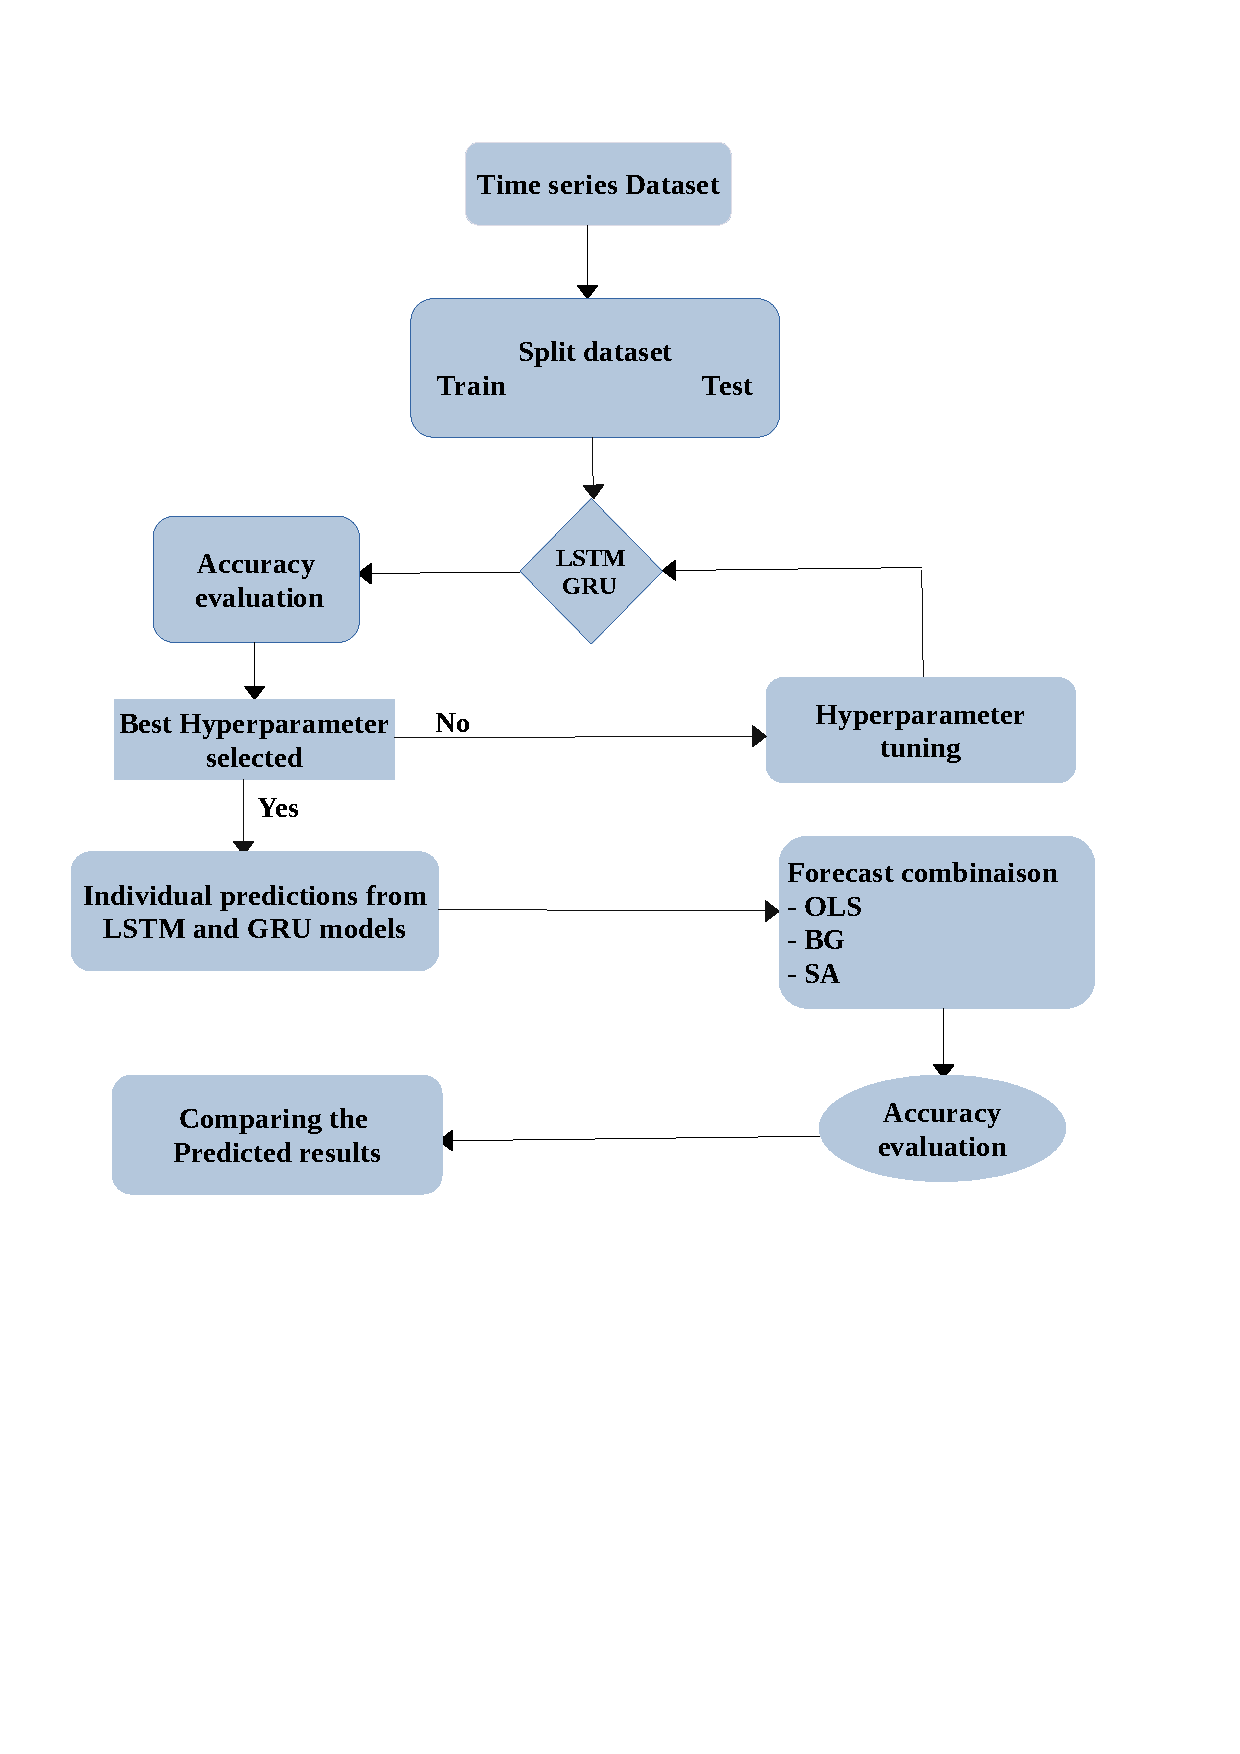
\includegraphics[scale=0.8]{method.pdf}
\caption{Overview of the forecasting combinaison system.}\label{method}
\end{figure}

\section{Empirical Results}
\subsection{Data and descriptive statistics}
In this study, we use the three leading cryptocurrencies by market capitalization: Bitcoin (BTC), Ethereum (ETH), and Litecoin (LTC). The dataset comprises daily closing prices sourced from \href{https://coinmarketcap.com}{CoinMarketCap} , covering the period from January 1, 2018, to March 22, 2025.  \autoref{ts} illustrates the temporal evolution of these three time series, highlighting key trends and volatility patterns over the observed timeframe.
\begin{figure}[H]
\centering 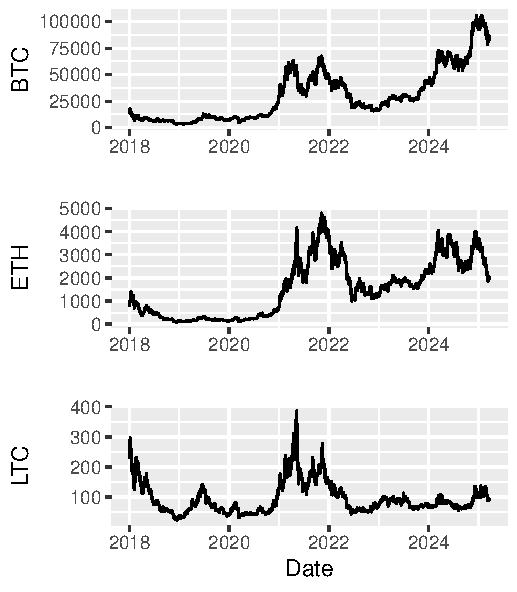
\includegraphics[scale=1.5]{ts.pdf}
\caption{BTC, ETH and LTC time series}\label{ts}
\end{figure}
The descriptive statistics for the daily closing prices of Bitcoin (BTC), Ethereum (ETH), and Litecoin (LTC) are summarized in \autoref{statDes}. Key metrics include measures of central tendency (mean, median), dispersion (standard deviation), and distributional properties (skewness, kurtosis), providing a comprehensive overview of the price dynamics across the study period.
\begin{table}[ht]
\centering
\begin{tabular}{llllllll}
  \hline
 & min & max & median & mean & std.dev & skewness & kurtosis \\ 
  \hline
BTC & 3236.762 & 106146.263 & 23175.891 & 30098.419 & 24624.704 & 1.027 & 0.353 \\ 
  ETH & 84.308 & 4812.088 & 1561.749 & 1549.258 & 1234.662 & 0.454 & -0.965 \\ 
  LTC & 23.464 & 386.451 & 77.263 & 94.459 & 52.309 & 1.627 & 3.131 \\ 
   \hline
\end{tabular}
\caption{Descriptive statistics} 
\label{statDes}
\end{table}
\subsection{Pre-processing}
\autoref{method} outlines the pre-processing pipeline applied to the cryptocurrency dataset to ensure compatibility with deep learning architectures, including LSTM and GRU.  Given the sensitivity of deep learning models to feature scales, we applied MinMax normalization to rescale the data into a $[0, 1]$ range, mitigating bias from disparate variable magnitudes. This approach aligns with established practices in time-series forecasting, where feature-wise scaling has been shown to enhance model convergence and performance \citep{ahsan2021}.
To evaluate model generalizability, we partitioned the dataset using an 90:10 training-test split, preserving temporal continuity—a critical consideration for autoregressive forecasting tasks. The pre-processed data was then restructured into sequences to facilitate supervised learning with recurrent neural networks (RNNs).
\subsection{Hyperparameter tuning}
The performance of Long Short-Term Memory (LSTM) and Gated Recurrent Unit (GRU) networks in time series forecasting heavily depends on careful hyperparameter selection. Our study employs random search optimization to efficiently navigate the hyperparameter space and identify configurations that enhance predictive accuracy. This method systematically evaluates combinations of critical parameters including network depth (number of layers), model capacity (hidden units), training dynamics (learning rate and batch size), regularization (dropout rate), and temporal context (sequence length).
\begin{table}[H]
\centering
\begin{tabular}{lc}
  \hline
  Hyperparameter & Range/Values \\ 
  \hline
   Number of layers & 1 to 5 (integer) \\ 
   Number of units & 32 to 512 (Increments of 32) \\ 
   Learning rate & 0.0001, to 0.01 (Logarithmic scale) \\ 
  Dropout rate & 0.1 to 0.5 (Increments of 0.1) \\ 
  Dense activation & ['relu','sigmoid'] \\ 
   \hline
\end{tabular}
\caption{Hyperparameter search space}\label{Hyp_ss}
\end{table}
Compared to exhaustive grid search, this approach offers superior computational efficiency by randomly sampling parameter combinations within predefined bounds while maintaining competitive model performance. Our implementation follows a structured workflow: first establishing parameter bounds (detailed in \autoref{Hyp_ss}), then iteratively training and evaluating models using validation sets. We employ standard regression metrics - Mean Squared Error (MSE) and Mean Absolute Error (MAE) - to objectively compare model variants.

The optimization process culminates in selecting the top-performing configuration for final evaluation. This methodology provides an effective balance between thorough parameter exploration and practical computational requirements, making it particularly valuable for tuning complex recurrent architectures.
\subsection{Performance metrics}
To rigorously evaluate the performance of our proposed RNN algorithms, we employed three widely-adopted statistical metrics:
\begin{itemize}
\item Root Mean Squared Error (RMSE) - measuring the standard deviation of prediction errors:
\begin{equation}
RMSE = \sqrt{\dfrac{\displaystyle{\sum_{i=1}^n \left(y_i-\widehat{y}_i\right)^2}}{n} }
\end{equation}
\item Root Mean Absolute Error (RMAE) - assessing average error magnitude:
\begin{equation}
RMAE =\sqrt{\dfrac{\displaystyle{\sum_{i=1}^n} \left|y_i-\widehat{y}_i\right| }{n } } 
\end{equation}
\item Mean Absolute Percentage Error (MAPE) - expressing accuracy as a percentage:
\begin{equation}
MAPE = \dfrac{100}{n}\sum_{i=1}^n \dfrac{|y_i-\widehat{y}_i|}{ai}
\end{equation} 
Where \(y_i\) represents the  actual value (observed) , \(\widehat{y}_i\) denotes the predicted value, and \(n\) stands for the total number of time steps.
\end{itemize}
These carefully selected metrics provide complementary perspectives on prediction accuracy. RMSE emphasizes larger errors through squaring, making it particularly sensitive to significant deviations. RMAE offers a more balanced view of typical error magnitudes, while MAPE provides an intuitive, scale-independent measure expressed as a percentage.
\subsection{Results and discussion}
The performance of various models in predicting the prices of Bitcoin (BTC), Ethereum (ETH), and Litecoin (LTC) is summarized in \autoref{metrics}, with the optimal model identified based on the smallest error metrics.
\begin{figure}[t]
\centering
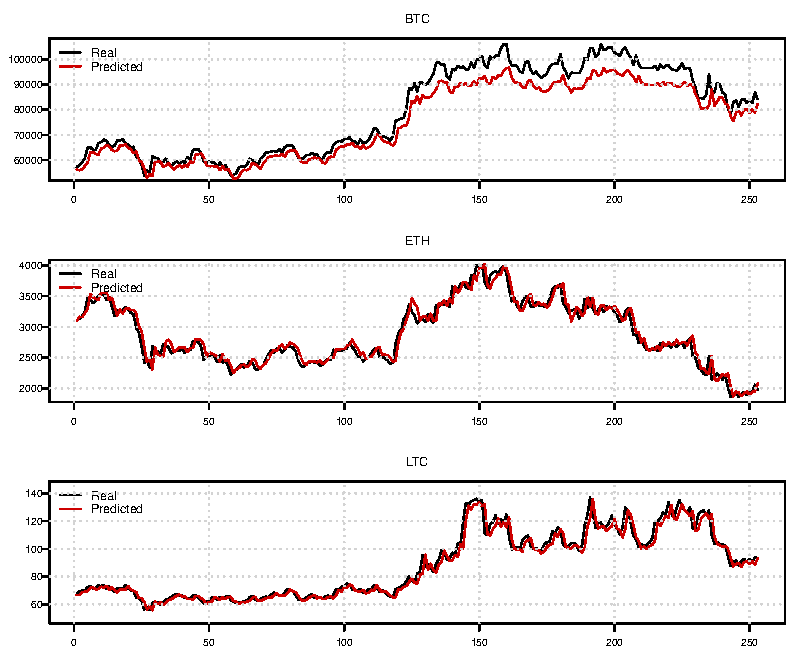
\includegraphics[scale=1.25]{LSTM.pdf}
\caption{Actual and predicted values using LSTM model}\label{lstm_res}
\end{figure}

\begin{figure}[t]
\centering
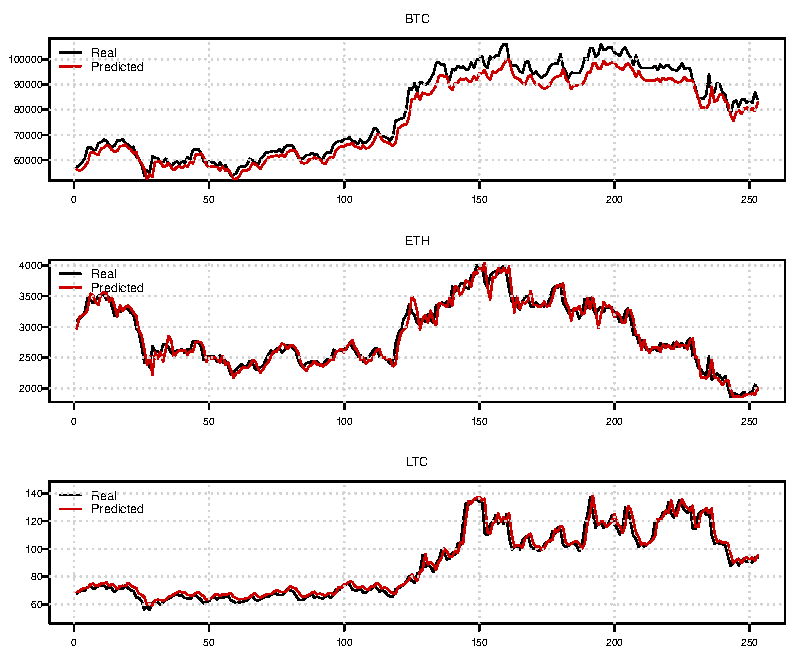
\includegraphics[scale=1.25]{GRU_.pdf}
\caption{Actual and predicted values using GRU model}\label{gru_res}
\end{figure}

\begin{figure}[t]
\centering
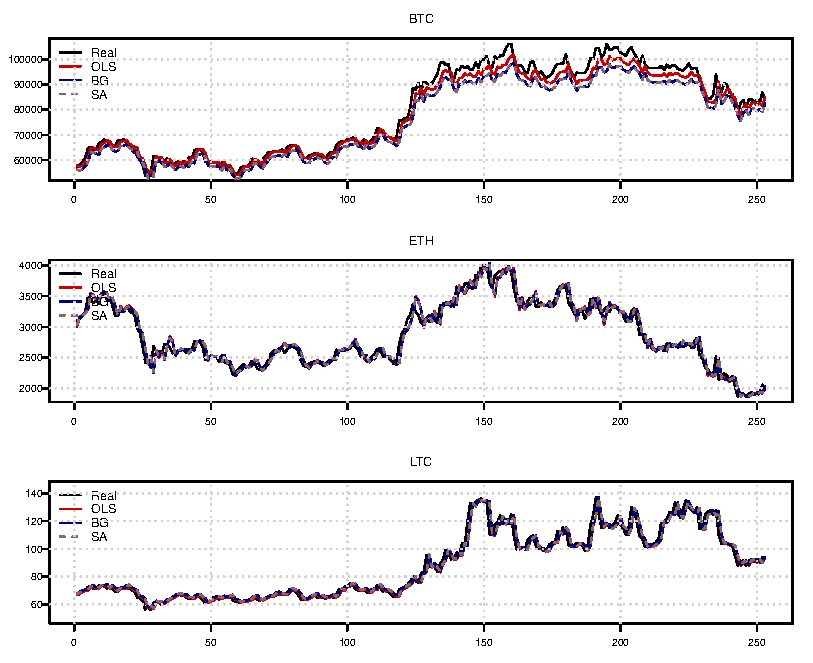
\includegraphics[scale=1.25]{comb_all.pdf}
\caption{Actual and predicted values using different combinaison  models}\label{comb_res}
\end{figure}

A visual comparison between the actual prices and the predicted values generated by the LSTM and GRU models is presented in \autoref{lstm_res} and \autoref{gru_res}, respectively. Additionally, \autoref{comb_res} illustrates the forecasts produced by different hybrid forecasting approaches. The plots demonstrate that the predicted values closely follow the actual trends, albeit with minor deviations. These discrepancies are further quantified by the performance metrics in \autoref{metrics}, providing a comprehensive assessment of each model's predictive accuracy.
\subsubsection{Results for BTC}
According to \autoref{metrics}, the combined Ordinary Least Squares (OLS) model outperforms all others in predicting BTC prices, achieving the lowest RMSE, RMAE, and MAPE values. This superiority is visually confirmed in \autoref{comb_res}, where the combined OLS predictions closely align with actual price movements, demonstrating high accuracy.

The results indicate that the combined OLS approach is more effective at capturing BTC trends than LSTM and GRU models, though the GRU remains competitive with only a marginal performance gap. Notably, the GRU model ranks second for BTC forecasting, exhibiting slightly elevated RMSE, RMAE, and MAPE values compared to OLS.

Overall, these findings suggest that hybrid statistical approaches (like combined OLS) surpass pure RNN-based methods (LSTM/GRU) in BTC price prediction, likely due to their robustness in handling linear trends and volatility.
\subsubsection{ Results for ETH}
The analysis of \autoref{metrics} and \autoref{lstm_res} reveals that the LSTM model delivers the best performance in forecasting Ethereum (ETH) prices, achieving the lowest error metrics—an RMSE of 114.52 and an RMAE of 9.216. \autoref{lstm_res} further supports this finding, demonstrating that the LSTM model’s predictions exhibit the smallest deviation from actual ETH prices, highlighting its superior accuracy.

However, when evaluating forecast precision based on MAPE (2.987), the combined simple average model emerges as the top performer, suggesting its advantage in percentage error minimization.

The LSTM model’s high predictive accuracy is also evident in Figure 16, where its forecasted ETH prices closely track the actual values throughout the testing period. The minimal discrepancies, as reflected by the low RMSE and RMAE, reinforce its reliability.

That said, a comparative assessment indicates that while the LSTM model outperforms GRU, its accuracy margin over combined models is relatively narrow, implying that hybrid approaches remain competitive alternatives for ETH price forecasting.
\begin{table}[t]
\centering
\caption{Forecasting quality metrics for different methods}\label{metrics}
\begin{tabular}{lccc|ccc}
%\toprule
\hline
\multicolumn{1}{c}{ } & \multicolumn{3}{c}{Train} & \multicolumn{3}{c}{Test} \\
%\cmidrule(l{3pt}r{3pt}){2-4} \cmidrule(l{3pt}r{3pt}){5-7}
\hline
 & RMSE & RMAE & MAPE & RMSE & RMAE & MAPE\\ \hline
%\midrule
%\addlinespace[0.3em]
\multicolumn{7}{l}{\textbf{BTC}}\\
\hspace{1em}LSTM & 1390.264 & 31.308 & 4.563 & 5358.839 & 66.428 & 5.114\\
\hspace{1em}GRU & 1308.704 & 28.497 & 3.073 & 4311.471 & 59.87 & 4.282\\
\hspace{1em}Comb\_OLS & \textbf{1033.683} & \textbf{24.165} &\textbf{ 2.396} & \textbf{2987.408} & \textbf{47.695} & \textbf{2.693}\\
\hspace{1em}Comb\_BG & 1340.918 & 29.712 & 3.662 & 4786.434 & 63.029 & 4.672\\
\hspace{1em}Comb\_SA & 1343.37 & 29.799 & 3.709 & 4818.105 & 63.227 & 4.697\\ \hline
%\addlinespace[0.3em]
\multicolumn{7}{l}{\textbf{ETH}}\\
\hspace{1em}LSTM & 74.317 & 7.253 & 8.811 & \textbf{114.527} & \textbf{9.216} & 2.99\\
\hspace{1em}GRU & 62.238 & 6.376 & 4.426 & 125.011 & 9.693 & 3.264\\
\hspace{1em}Comb\_OLS & \textbf{59.769} & \textbf{6.114} & \textbf{4.288} & 120.632 & 9.469 & 3.115\\
\hspace{1em}Comb\_BG & 62.258 & 6.478 & 5.764 & 117.045 & 9.313 & 3.018\\
\hspace{1em}Comb\_SA & 63.24 & 6.556 & 6.15 & 115.978 & 9.262 & \textbf{2.987}\\ \hline
%\addlinespace[0.3em]
\multicolumn{7}{l}{\textbf{LTC}}\\
\hspace{1em}LSTM & 6.586 & 1.948 & 3.781 & 4.845 & 1.792 & 3.341\\
\hspace{1em}GRU & 6.118 & 2.02 & 4.749 & 4.977 & 1.856 & 3.81\\
\hspace{1em}Comb\_OLS &\textbf{ 5.801} & \textbf{1.845} & \textbf{3.424} & 4.728 & \textbf{1.755} & \textbf{3.214}\\
\hspace{1em}Comb\_BG & 5.974 & 1.914 & 3.981 & 4.698 & 1.758 & 3.261\\
\hspace{1em}Comb\_SA & 5.99 & 1.91 & 3.941 & \textbf{4.691} & \textbf{1.755} & 3.244\\ \hline
%\bottomrule
\end{tabular}
\end{table}
\subsubsection{Results for LTC}
\autoref{metrics} presents a comprehensive evaluation of model performance for Litecoin (LTC) price prediction, revealing distinct advantages among competing approaches. The combined Ordinary Least Squares (OLS) model emerges as particularly effective, achieving the lowest error metrics with an RMAE of 1.755 and MAPE of 3.214, indicating superior predictive accuracy among all tested models. However, the combined simple average model demonstrates the best performance in terms of RMSE (4.691), suggesting particular strength in minimizing large prediction errors. Visual analysis through \autoref{lstm_res, gru_res, comb_res} provides compelling graphical evidence of these quantitative findings. \autoref{lstm_res} highlights the LSTM model's strong performance, with its predictions closely tracking actual LTC prices as evidenced by excellent error metrics (MAPE: 3.341; RMSE: 1.792). The combined OLS model's results, depicted in \autoref{comb_res}, show marginally better performance than LSTM in percentage terms (MAPE: 3.214; RMAE: 1.755), though the visual representation suggests the practical differences between these top-performing models are relatively minor. This nuanced interpretation of both tabular and graphical data confirms that while statistical hybrids like combined OLS show theoretical advantages, advanced neural network approaches (LSTM/GRU) remain highly competitive for LTC forecasting.
\section{Conclusions}
This study systematically evaluates hybrid models integrating RNNs (LSTM and GRU) with statistical techniques for cryptocurrency price prediction. Key findings highlight the superiority of the combined OLS model for BTC and LTC, attributed to its ability to harmonize linear trends with deep learning’s nonlinear pattern recognition. For ETH, LSTM’s temporal modeling prowess yields the most accurate forecasts, though hybrid methods remain competitive. The results emphasize three critical insights:

\textbf{Hybrid Superiority}: Combining RNNs with statistical methods (e.g., OLS) enhances robustness, particularly for highly volatile assets like BTC.

\textbf{Asset-Specific Performance}: Model efficacy varies by cryptocurrency, suggesting tailored approaches—LSTM for ETH’s complex dynamics, OLS hybrids for BTC/LTC’s trends.

\textbf{Practical Implications}: The minimal discrepancies between predicted and actual values (evidenced by low error metrics and visualizations) validate these models’ utility for real-world decision-making.

Future research could explore integrating exogenous variables (e.g., sentiment data) or ensemble techniques to further refine accuracy. By bridging statistical and deep learning paradigms, this work contributes a scalable framework for cryptocurrency forecasting, offering both academic and practical value in navigating decentralized financial markets.


%%%%%%%%%%%%%%%%%%%%%%%%%%%%%%%%%%%%%%%%%%%%%%%%%%%%%%
%          AI TOOLS, USE AND LOCATION
%%%%%%%%%%%%%%%%%%%%%%%%%%%%%%%%%%%%%%%%%%%%%%%%%%%%%%
%We follow COPE's guidelines and policies regarding the use of Artificial Intelligence (AI) tools. COPE Policy on AI tools can be found at https://publicationethics.org/cope-position-statements/ai-author.

%Authors using AI tools in the writing of a manuscript, production of images or graphical elements of the paper, or in the collection and analysis of data, must be transparent in disclosing in this section how the AI tool was used and which tool was used. Authors are fully responsible for the content of their manuscript, even those parts produced by an AI tool, and are thus liable for any breach of publication ethics. - COPE

%Disclosure instructions

%If there is nothing to disclose, there is no need to add a declaration, otherwise please declare.

%\section*{Use of AI tools declaration}
%The author(s) declare(s) they have used Artificial Intelligence (AI) tools in the creation of this article.
%AI tools used:
%How were the AI tools used?
%Where in the article is the information located?

\section*{Use of AI tools declaration}
The authors declare they have not used Artificial Intelligence (AI) tools in the creation of this article.

%\section*{Acknowledgments (All sources of funding of the study must be disclosed)}
%We would like to thank you for following the instructions above
%very closely in advance. It will definitely save us lot of \cite{oyewola2022}
%time and expedite the process of your paper's publication.
%\cite{artzner1999coherent}

%\section*{Conflict of interest}

%The authors declare all relationships, financial, commercial or otherwise, that might be perceived by the academic community as representing a potential conflict of interest. If there are no such relationships, the author can state “All authors declare no conflicts of interest in this paper” in this section.

\begin{thebibliography}{999}

\bibitem[Aghashahi, and Bamdad  2023]{aghashahi2023}
\newblock Aghashahi M and Bamdad S (2023)
\newblock Analysis of different artificial neural networks for Bitcoin price prediction. 
\newblock \emph{International Journal of Management Science and Engineering Management} 18(2): 126-133.

\bibitem[Ahsan, et al. 2021]{ahsan2021}
\newblock Ahsan M. M., Mahmud M. P., Saha P. K., Gupta K. D., and Siddique Z. (2021) 
\newblock Effect of data scaling methods on machine learning algorithms and model performance, \newblock \emph{Technologies} 9(3).

\bibitem[Amberkhani, et al. 2025]{amberkhani2025}
\newblock Amberkhani A, Bolisetty H, Narasimhaiah R, Jilani G, Baheri B, Muhajab H, Gharinour K,  and Shubbar S. (2025)
\newblock  Revolutionizing Cryptocurrency Price Prediction: Advanced Insights from Machine Learning, Deep Learning and Hybrid Models.
\newblock \emph{ In Future of Information and Communication Conference.}
\newblock Cham: Springer Nature Switzerland, 274-286.

\bibitem[Amirshahi, and Lahmiri  2025]{amirshahi2025}
\newblock Amirshahi B, and Lahmiri S (2025)
\newblock Investigating the effectiveness of Twitter sentiment in cryptocurrency close price prediction by using deep learning.
\newblock \emph{Expert Systems} 42(1).

\bibitem[Bates, and Granger 1969]{bates1969}
\newblock Bates J. M, and Granger C. W (1969) The combination of forecasts,
\newblock \emph{Journal of the operational research society} 20(4): 451-468.

\bibitem[Dudek,  2023]{dudek2023}
\newblock Dudek G (2023) Combining Forecasts of Time Series with Complex Seasonality Using LSTM-Based Meta-Learning,
\newblock \emph{Engineering Proceedings} 39(1).

\bibitem[Ferdiansyah, et al. 2023]{ferdiansyah2023}
\newblock Ferdiansyah F, Othman S. H, Radzi R. Z. M, Stiawan, D, and Sutikno, T (2023)
\newblock Hybrid gated recurrent unit bidirectional-long short-term memory model to improve cryptocurrency prediction accuracy.
\newblock \emph{ IAES International Journal of Artificial Intelligence} 12(1).

\bibitem[García-Medina, and Aguayo-Moreno 2024]{garcia2024}
\newblock García-Medina A and Aguayo-Moreno E (2024)
\newblock LSTM–GARCH hybrid model for the prediction of volatility in cryptocurrency portfolios. 
\newblock \emph{Computational Economics} 63(4): 1511-1542.

\bibitem[Hafidi, et al. 2025]{hadfi2025}
\newblock Hafidi N, Khoudi Z, Nachaoui M, and Lyaqini S. (2025)
\newblock Cryptocurrency Price Prediction with Genetic Algorithm-based Hyperparameter Optimization. 
\newblock \emph{Statistics, Optimization \& Information Computing}.

\bibitem[Hoa, et al. 2025]{hoa2025}
\newblock Hoa T. T, Le T. M, and Nguyen-Dinh, C. H. (2025)
\newblock Hybrid model of 1D-CNN and LSTM for forecasting Ethereum closing prices: a case study of temporal analysis.
\newblock \emph{ International Journal of Information Technology}: 1-13.
https://doi.org/10.1007/s41870-025-02472-6

\bibitem[Hochreiter,  and Schmidhuber 1997]{hochreiter97}
\newblock Hochreiter S, and Schmidhuber J (1997) Long short-term memory. 
\newblock \emph{Neural computation} 9(8): 1735-1780.

\bibitem[Kiranmai Balijepalli , and Thangaraj 2025]{kiranmai2025}
\newblock Kiranmai Balijepalli N. S. S, and Thangaraj V (2025)
\newblock Prediction of cryptocurrency’s price using ensemble machine learning algorithms.
\newblock \emph{European Journal of Management and Business Economics}
 https://doi.org/10.1108/EJMBE-08-2023-0244

\bibitem[Cho, et al. 2014]{chao2014}
\newblock  Cho K, Merrienboer B. V , Gulcehre C , Bahdanau D , Bougares F, Schwenk H, and Bengio Y (2014)
\newblock Learning Phrase Representations using RNN Encoder-Decoder for Statistical Machine Translation,
\newblock https://doi.org/10.48550/arXiv.1406.1078 

\bibitem[Oyewola, et al. 2022]{oyewola2022}
\newblock Oyewola D. O, Dada E. G, and Ndunagu J. N (2022)
\newblock A novel hybrid walk-forward ensemble optimization for time series cryptocurrency prediction. 
\newblock \emph{Heliyon} 8(11).

\bibitem[Seabe, et al. 2023]{seabe2023}
\newblock Seabe P. L, Moutsinga C. R. B. and Pindza E (2023)
\newblock Forecasting cryptocurrency prices using LSTM, GRU, and bi-directional LSTM: a deep learning approach, 
\newblock \emph{Fractal and Fractional} 7(2).

\bibitem[Vasilev, 2019]{vasilev2019}
\newblock Vasilev I (2019) Advanced Deep Learning with Python: Design and implement advanced next-generation AI solutions using TensorFlow and PyTorch,
\newblock \emph{ }
\newblock Packt Publishing
% https://books.google.tn/books?id=TxbEDwAAQBAJ

\bibitem[Xiang,  2024]{xiang2024}
\newblock Xiang Q (2024) Cryptocurrency assets valuation prediction based on LSTM, neural network, and deep learning hybrid model,
\newblock \emph{Applied and Computational Engineering} 49: 265-272.

\bibitem[Yang, et al. 2020]{yang2020}
\newblock Yang, Shudong and Yu, Xueying and Zhou, Ying (2020)
\newblock Lstm and gru neural network performance comparison study: Taking yelp review dataset as an example,
\newblock \emph{2020 International workshop on electronic communication and artificial intelligence (IWECAI)}:98-101.

\bibitem[Zhang, et al. 2021]{zhang2021}
\newblock Zhang Z, Dai H. N, Zhou J, Mondal S. K. García M. M., and Wang H (2021)
\newblock Forecasting cryptocurrency price using convolutional neural networks with weighted and attentive memory channels.
\newblock \emph{ Expert Systems with Applications} 183: 115378.

\end{thebibliography}

%\section*{Supplementary (if necessary)}

%We encourage authors to submit detailed supplementary, including dataset, document, image, video, software code, protocol, supporting information, table etc, but some large datasets ( $>$ 100 MB) should be deposited in specialized service providers by author. The supplementary should be submitted in a separated file.

\end{document}
